\documentclass{scrartcl}

\usepackage[utf8]{inputenc}
\usepackage[T1]{fontenc}
\usepackage{lmodern}
\usepackage[english]{babel}
\usepackage{amsmath}
\usepackage{graphicx}
\usepackage{caption}	
\usepackage{subcaption}	 
\usepackage{hyperref}
\usepackage[parfill]{parskip}
\usepackage{hhline}
\usepackage{subcaption}

\title{Neuroprosthetics - Exercise 4}
\author{Alexander Koenig}
\date{4. December 2019}

\begin{document}
\maketitle

\section{Time Constants and Steady-State Values}

\textbf{Derivation of Formulae}

The relationship between the voltage dependent rates $\alpha_x, \beta_x$ and the time constant $\tau_x$ (equation \ref{eq:tau}) and steady state value $x_\infty$ (equation \ref{eq:xinf}) with $x \in \{m, n, h\} $ can be derived from the gating equation in equation \ref{eq:gating}.

\begin{align}
	\label{eq:gating}
	\frac{dx}{dt} &= [\alpha_x(1-x) - \beta_x x]\cdot k \\
	\frac{dx}{dt} &= [\alpha_x -\alpha_x x - \beta_x x]\cdot k \\
	\frac{dx}{dt} &= [\alpha_x - (\alpha_x + \beta_x)\cdot x]\cdot k \\
	\frac{dx}{dt} &= (\frac{\alpha_x}{\alpha_x + \beta_x} - x) \cdot (\alpha_x + \beta_x)\cdot k \\
	\frac{dx}{dt} &= \frac{1}{\tau_x} (x_\infty - x)
	\intertext{with}
	\label{eq:tau} \tau_x &= \frac{1}{(\alpha_x + \beta_x)\cdot k} \\
	\label{eq:xinf} x_\infty &= \frac{\alpha_x}{\alpha_x + \beta_x} \\
	\intertext{and the temperature correction factor}
	\label{eq:k} k&=3^{0.1(T-6.3)} 
\end{align}

\newpage
\textbf{Interpretations of Plots}

Figures \ref{fig:tau_temp6.3} and \ref{fig:tau_temp28} show the relationship between the membrane potential and the time constants $\tau_x$. The time constants represent the time needed for the gates to approach their steady state values $x_\infty$ at a specific membrane potential. The steady state values are approached exponentially (see definition of $\alpha_x$ and $\beta_x$ in section \ref{HH}). 

When figures \ref{fig:tau_temp6.3} and \ref{fig:tau_temp28} are compared a temperature dependency becomes evident. At higher temperatures, the time constants $\tau_x$ are shorter for all membrane potentials and hence the steady-state values $x_\infty$ are approached sooner. Vice versa, it takes longer to approach the steady-state values of the gating variables if the temperature is lower. This is because the temperature is inversely proportional to the time constant which is evident from equations \ref{eq:tau} and \ref{eq:k}. 

It is clear that the $m$ gate (sodium activation gate) has the smallest time constants and hence can approach its steady-state value the fastest. This corresponds to the well-known fact that sodium channels are very quick to activate and deactivate. It takes the $n$ gate (potassium activation gate) longer to approach the steady-state value than the $m$ gate. The $h$ gate (sodium inactivation gate) is the slowest of all gates at resting potential (V = 0mV $\pm$ 15mV). However, for higher or lower membrane potentials the $h$ gate is faster than the $n$ gate but still slower than the $m$ gate. These observations are valid for both temperatures. 

Figures \ref{fig:xinf_temp6_3} and \ref{fig:xinf_temp28} show the relationships between the membrane potential and the steady state values for the gating variables at different temperatures. Since $x_\infty$ is not temperature dependent both plots are identical. Note that equations \ref{eq:sodium} and \ref{eq:potassium} model the sodium and potassium channels respectively. 

For strongly negative membrane potentials the sodium inactivation gate is fully opened ($P_{open} \approx 1$) but both sodium and potassium activation gates are closed ($P_{open} \approx 0$). Hence no sodium or potassium current can flow (refer to equations \ref{eq:sodium} and \ref{eq:potassium}). At resting potential ($V_{rest} = 0$) the sodium channels are nearly completely closed ($m_\infty=0.05$ and $h_\infty=0.60$) while a few potassium channels are open ($n_\infty=0.32$). When the cell begins to \underline{depolarize} and the membrane potential rises, more sodium and potassium channels open. The sodium channels open faster than the potassium channels because $\tau_m$ is much smaller than $\tau_n$. As observed earlier the sodium inactivation gates are especially slow in the region of the resting potential and hence the depolarization can continue - an action potential occurs. When the membrane potential rises further the sodium and potassium activation gates are fully opened ($P_{open} \approx 1$) whereas the sodium inactivation gate is fully closed ($P_{open} \approx 0$). As a result, no further inflow of sodium ions is possible, but potassium ions can still flow out of the cell. The cell \underline{repolarizes} and both ion channels start to close. Because the potassium channels close slower than the sodium channels even more potassium ions can flow out of the cell. The cell enters the \underline{hyperpolarization} phase before it recovers back to the resting potential.

\newpage
\begin{figure}[h]
	\centering
	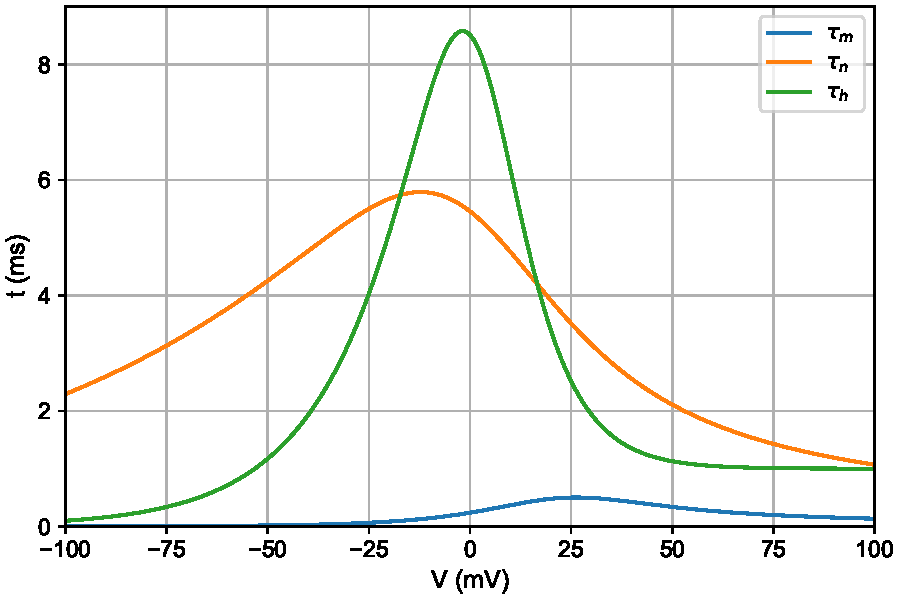
\includegraphics[width=0.9\textwidth]{figures/tau_temp6.3.pdf}
	\caption{Time constants for temperature 6.3 $^{\circ}$C}
	\label{fig:tau_temp6.3}
\end{figure}
\begin{figure}[h!]
	\centering
	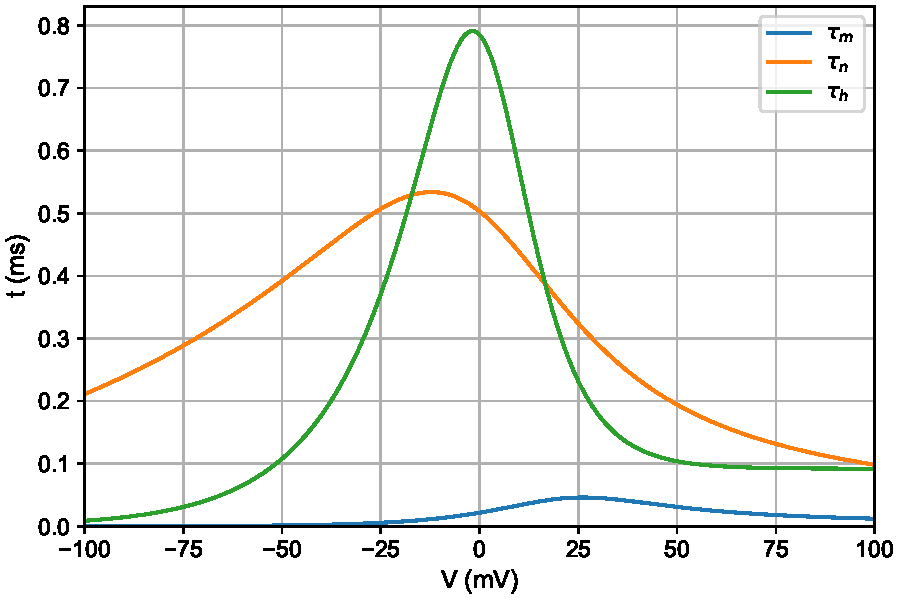
\includegraphics[width=0.9\textwidth]{figures/tau_temp28.pdf}
	\caption{Time constants for temperature 28 $^{\circ}$C}
	\label{fig:tau_temp28}
\end{figure}

\newpage
\begin{figure}[h]
	\centering
	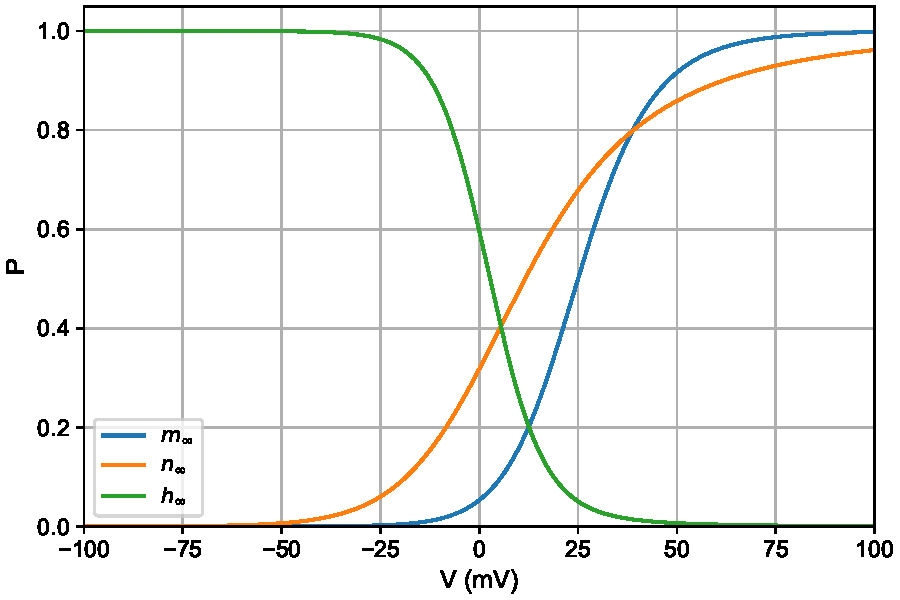
\includegraphics[width=0.9\textwidth]{figures/xinf_temp6.3.pdf}
	\caption{Steady state values for temperature 6.3 $^{\circ}$C}
	\label{fig:xinf_temp6_3}
\end{figure}
\begin{figure}[h!]
	\centering
	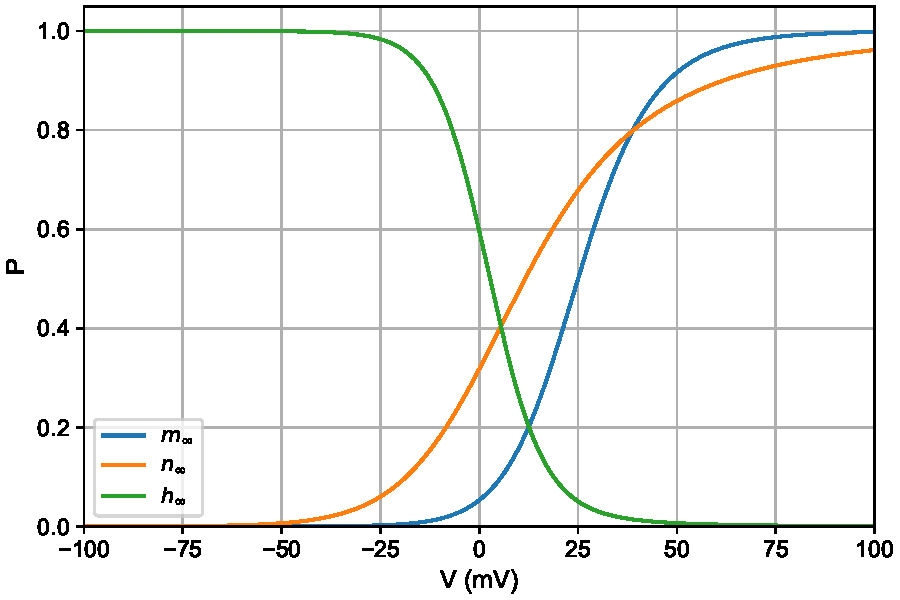
\includegraphics[width=0.9\textwidth]{figures/xinf_temp28.pdf}
	\caption{Steady state values for temperature 28 $^{\circ}$C}
	\label{fig:xinf_temp28}
\end{figure}

\newpage
\section{Hodgkin-Huxley Neuron Model}\label{HH}
By conducting voltage-clamp experiments to investigate the squid giant axon Hodgkin and Huxley formulated a mathematical model that describes the formation and propagation of action potentials. The model is governed by four nonlinear differential equations that represent the electrical characteristics of excitable cells. Equation \ref{eq:membrane} models the potential across the cell membrane and equations \ref{eq:m}, \ref{eq:n} and \ref{eq:h} describe the behaviour of the gating variables. All constants and units are used as in the original publication by Hodgkin and Huxley. 

\begin{align}
\frac{d V}{d t}&=\frac{1}{c}\left(-i_{i o n}+i_{s t i m u l u s}\right) \label{eq:membrane} \\
\frac{d m}{d t}&=\left[\alpha_{m}(1-m)-\beta_{m} m\right] k \label{eq:m}\\
\frac{d n}{d t}&=\left[\alpha_{n}(1-n)-\beta_{n} n\right] k \label{eq:n}\\
\frac{d h}{d t}&=\left[\alpha_{h}(1-h)-\beta_{h} h\right] k \label{eq:h}\\
\intertext{with the ion currents}
i_{i o n}&=i_{N a}+i_{K}+i_{L} \\
i_{N a}&=\bar{g}_{N a} m^{3} h\left(V-V_{N a}\right) \label{eq:sodium}\\
i_{K}&=\bar{g}_{K} n^{4}\left(V-V_{K}\right) \label{eq:potassium}\\
\label{eq:il}i_{L}&=\bar{g}_{L}\left(V-V_{L}\right) \\
\intertext{and the rate equations}
\alpha_{m} &=\frac{2.5-0.1 V}{e^{(2.5-0.1 V)}-1} \\ 
\alpha_{n} &=\frac{0.1-0.01 V}{e^{(1-0.1 V)}-1} \\ 
\alpha_{h} &=0.07 e^{-V / 20} \\
\beta_{m} &=4 e^{-V / 18} \\ 
\beta_{n} &=0.125 e^{-V / 80} \\ 
\beta_{h} &=\frac{1}{e^{(3-0.1 V)}+1}
\end{align}


In this exercise the stimulating current $i_{s t i m u l u s}$ consists of five 5ms long rectangular pulses with a gap of 10ms and the amplitudes 1$\mu$A, 2$\mu$A, 3$\mu$A, 4$\mu$A, 5$\mu$A for 6.3 $^{\circ}$C and 2$\mu$A, 4$\mu$A, 8$\mu$A, 16$\mu$A, 32$\mu$A for 28 $^{\circ}$C respectively. The stimulating currents are displayed in figures \ref{fig:inputcur_temp6_3} and \ref{fig:inputcur_temp28}.
\newpage

\textbf{Difference between Temperatures}

\underline{Membrane Potential}: The amplitude of the spikes in figure \ref{fig:potential_temp6_3} is larger than in figure  \ref{fig:potential_temp28} even though the stimulation current is  higher. We conclude from this that higher stimulation currents are needed at higher temperatures to generate an action potential. This is due to the more rapid opening and closing of ion channels at higher temperatures. Another observation that relates to this is that each stimulus leads to exactly one action potential in figure \ref{fig:potential_temp6_3} whereas one stimulus can produce multiple spikes in figure \ref{fig:potential_temp28}. Hence the membrane potential spikes in a more regular pattern for the lower temperature.

\underline{Gating Variables}: The gating variables tend towards their steady state values ($m_\infty=0.05$, $h_\infty=0.60$, $n_\infty=0.32$) faster at higher temperatures. As a result more action potentials can be released with one stimulus. At the higher temperature the gates are also more responsive to the stimuli that do not elicit an action potential (i.e. at $t \in \{0ms, 5ms\}$, $t \in \{15ms, 20ms\}$ and $t \in \{30ms, 35ms\}$). 

\underline{Ion Currents}: The amplitude of the potassium and sodium currents is slightly reduced by the temperature increase. The current spikes correspond to the action potentials (with the sodium current rising slightly earlier than the potassium current as the sodium gates open quicker). The sodium currents are negative (cations flow into the cell) whereas the potassium currents are positive (cations flow out of the cell). 

\textbf{Generation of an Action Potential}

An action potential is a large spike in the membrane potential of a neuron. The generation of action potentials is best explained by investigating the behavior of the gating variables for sodium and potassium in figure \ref{fig:gatingvars_temp6_3}. 

A stimulation current of 1 $\mu$A and 2 $\mu$A slightly rises the membrane potential in the interval $t \in \{0ms, 5ms\}$ and $t \in \{15ms, 20ms\}$ but is not sufficient to overcome the threshold voltage (see figure \ref{fig:potential_temp6_3}). However, a stimulus of 3 $\mu$A in the interval $t \in \{30ms, 35ms\}$ is sufficient to overcome this threshold, which activates both sodium and potassium channels through the $m$ and $n$ gates. But the sodium channels $m$ open much faster than the potassium channels due to the lower time constant $\tau_m$. The inflow of positively charged sodium ions leads to a positive feedback loop and further depolarizes the cell as more sodium channels are opened. The rapid opening of the sodium activation gates ($m$ gates) is displayed in figure \ref{fig:gatingvars_temp6_3} and the high sodium currents are shown in figure \ref{fig:currents_temp6_3}.

As the membrane potential increases further the slow potassium gates $n$ open, the potassium outflow increases, and the sodium channels are deactivated as the sodium inactivation gate $h$ tends towards 0 in figure \ref{fig:gatingvars_temp6_3}). When the net outflow of potassium ions exceeds the inflow of sodium ions the membrane potential starts to repolarize back to the resting potential. Since the potassium channels are slow to close more potassium ions flow out of the cell and the potential undershoots, which is known as hyperpolarization. The cell's membrane potential is restored to the resting potential when the sodium inactivation gate $h$ returns to its steady-state value. If the membrane potential reaches the threshold voltage again another action potential can be elicited. 

\textbf{Amplitude Decrease of Action Potentials at 28 $^{\circ}$C}

This effect can be explained by investigating the gating variables displayed in figure \ref{fig:closeup_temp28}. The reason for the amplitude decrease of the action potentials at 28 $^{\circ}$C is that the relative refractory period is not yet overcome before a new action potential starts to form. The slow potassium channels $n$ cannot return to their steady-state value of approximately 0.32 before the cell depolarizes again. The reduced membrane potential during hyperpolarization leads to an increase in the necessary current to lift the potential above the firing threshold again to elicit another action potential. However, since the stimulation current is constant at 32 $\mu$A in the investigated time frame the amplitude of the resulting action potential decreases.

\textbf{Interpretation of Phase Plots}

Phase plots are an invaluable tool when evaluating dynamical systems as they represent the directional behavior of a system of differential equations. Phase plots can be used to analyze the stability of a dynamic system. 

The phase plots in figures \ref{fig:phase_temp6_3} and \ref{fig:phase_temp28} display the relationship between the transmembrane potential and the ion and leakage currents. The state of the dynamical system is described by a tuple of voltage and current. The evolution rule describes what future states can follow from the current state. The trajectories in the plots visualize these voltage/current tuples that occurred in the time frame of the simulation. 

As the membrane potential rises/falls the leakage current increases/decreases on a linear trajectory for both temperatures. This is also evident from equation \ref{eq:il} as the current $i_L$ linearly depends on $V$. The behavior of the sodium and potassium trajectories is more complex. Since the amplitudes of the sodium and potassium currents at 6.3$^\circ$C are almost identical for each action potential the trajectories lie very close together in figure \ref{fig:phase_temp6_3}. For 28$^\circ$C the amplitudes of the sodium and potassium currents are not identical (see figure \ref{fig:currents_temp28}) and hence the trajectories lie further apart in figure \ref{fig:phase_temp28}. The sharper edges of the sodium current/voltage trajectory at 6.3$^\circ$C are due to the faster opening and closing of the sodium gates. As sodium currents are negative the sodium trajectories lie in the bottom half of the plot in both cases (vice versa for the potassium trajectories).

\textbf{Comparison LIF and HH Model}

The simple leaky integrate and fire (LIF) neuron does not model the ion pump and sets the resting potential by a battery in its equivalence circuit. The LIF model cannot actively produce action potentials and hence a stimulation current has to be introduced. The benefits of the LIF model are that it is computationally lightweight and suffices to model simple questions regarding neuronal behavior. 

In comparison, the Hodkin-Huxley (HH) model is a more sophisticated model that is more biophysically meaningful. It models the ion pump and can produce action potentials. Therefore it is suitable to model more complex neuronal behavior. However, this comes at a higher computational cost.

\newpage
\begin{figure}[h]
	\centering
	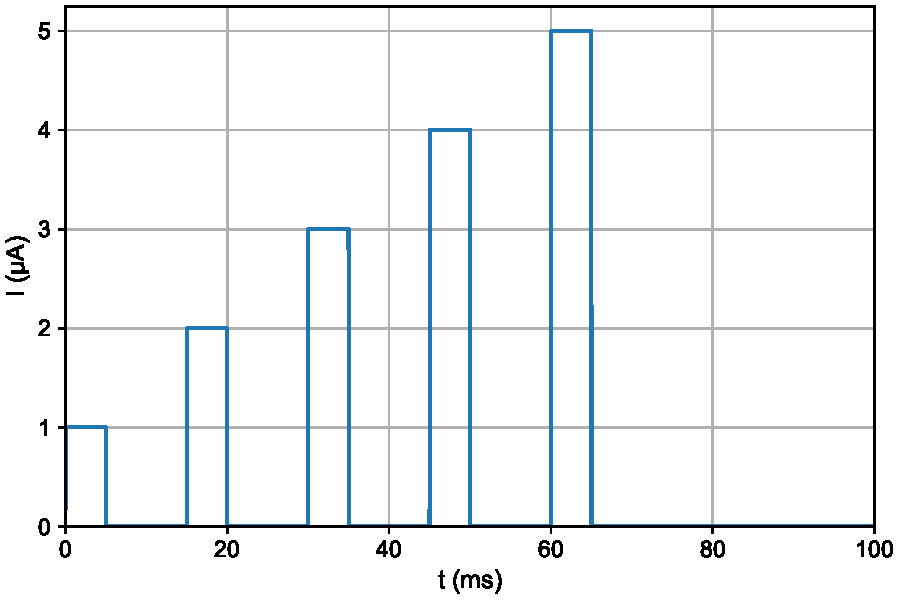
\includegraphics[width=0.9\textwidth]{figures/inputcur_temp6.3.pdf}
	\caption{Stimulation current for temperature 6.3 $^{\circ}$C}
	\label{fig:inputcur_temp6_3}
\end{figure}
\begin{figure}[h!]
	\centering
	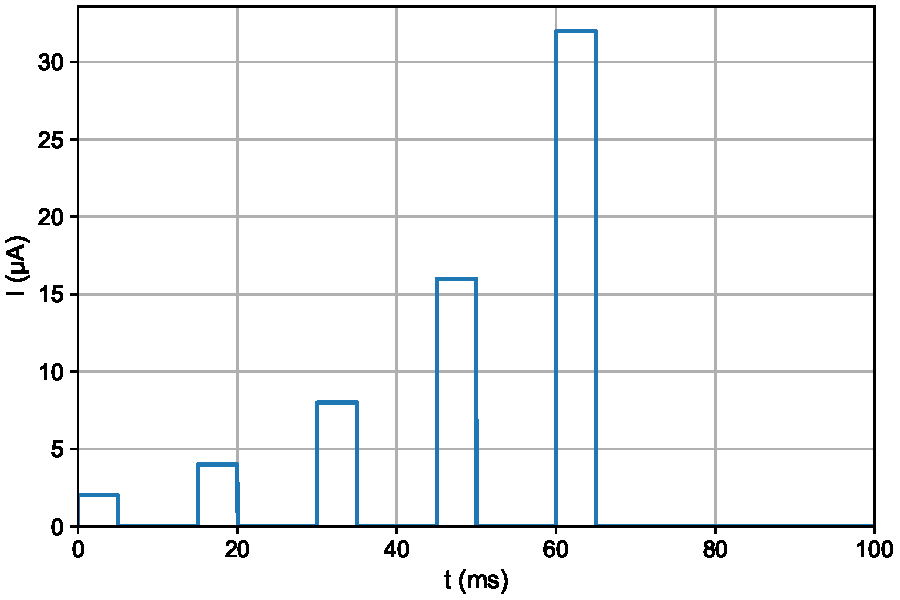
\includegraphics[width=0.9\textwidth]{figures/inputcur_temp28.pdf}
	\caption{Stimulation current for temperature 28 $^{\circ}$C}
	\label{fig:inputcur_temp28}
\end{figure}

\newpage
\begin{figure}[h]
	\centering
	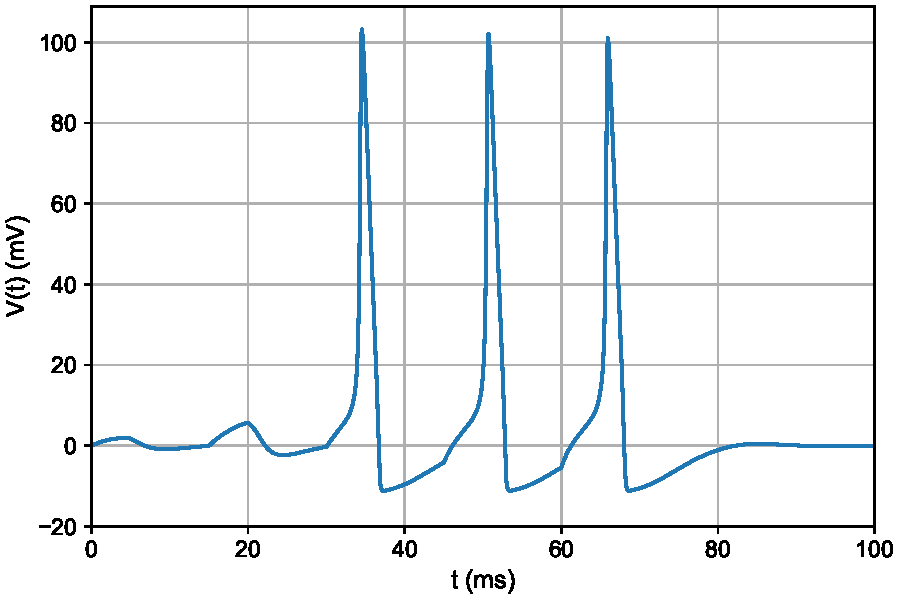
\includegraphics[width=0.9\textwidth]{figures/potential_temp6.3.pdf}
	\caption{Membrane potential for temperature 6.3 $^{\circ}$C}
	\label{fig:potential_temp6_3}
\end{figure}
\begin{figure}[h!]
	\centering
	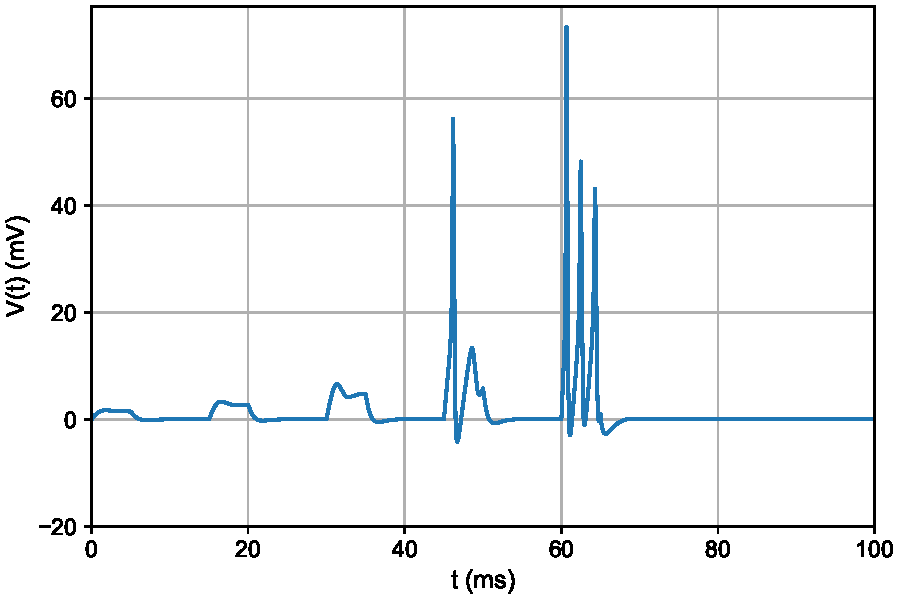
\includegraphics[width=0.9\textwidth]{figures/potential_temp28.pdf}
	\caption{Membrane potential for temperature 28 $^{\circ}$C}
	\label{fig:potential_temp28}
\end{figure}

\newpage
\begin{figure}[h]
	\centering
	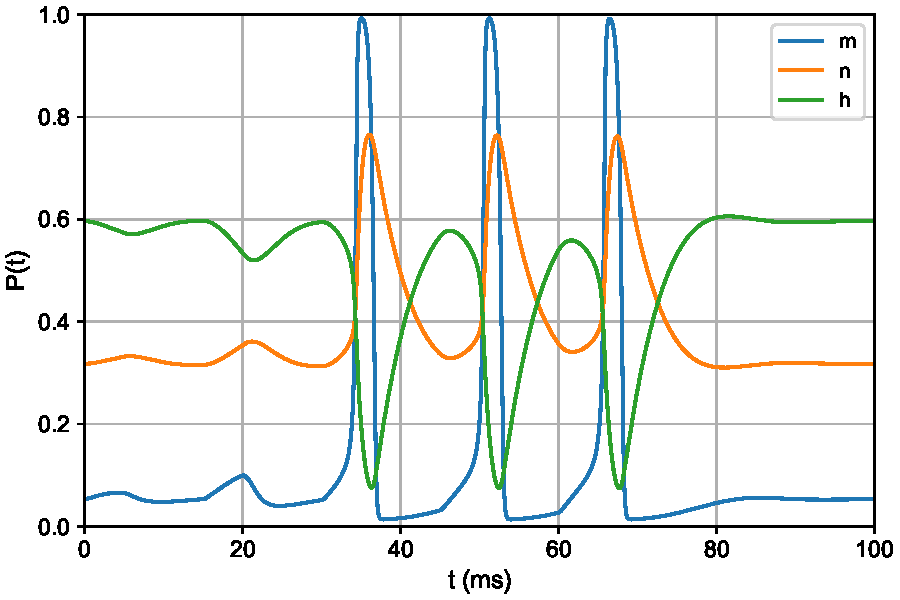
\includegraphics[width=0.9\textwidth]{figures/gatingvars_temp6.3.pdf}
	\caption{Gating variables for temperature 6.3 $^{\circ}$C}
	\label{fig:gatingvars_temp6_3}
\end{figure}
\begin{figure}[h!]
	\centering
	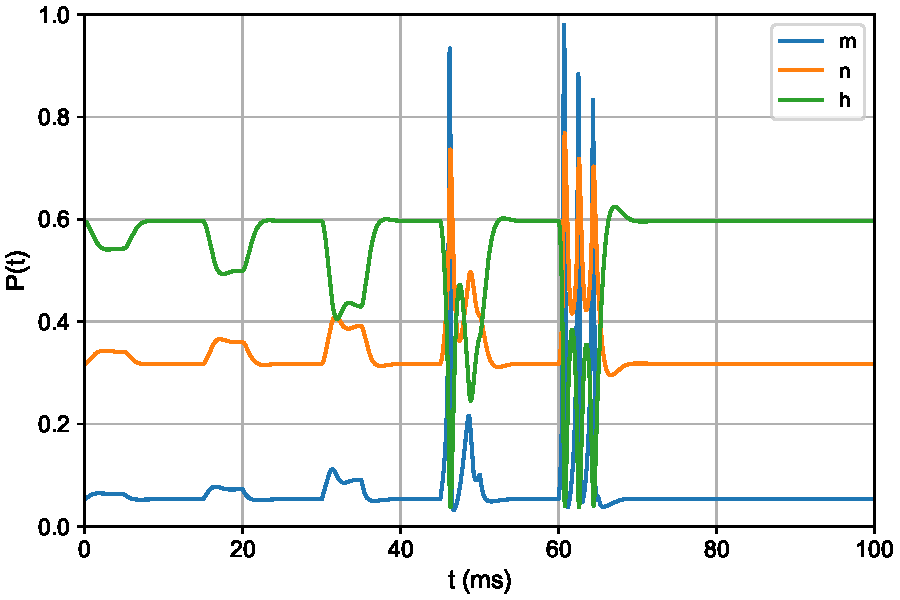
\includegraphics[width=0.9\textwidth]{figures/gatingvars_temp28.pdf}
	\caption{Gating variables for temperature 28 $^{\circ}$C}
	\label{fig:gatingvars_temp28}
\end{figure}

\newpage
\begin{figure}[h]
	\centering
	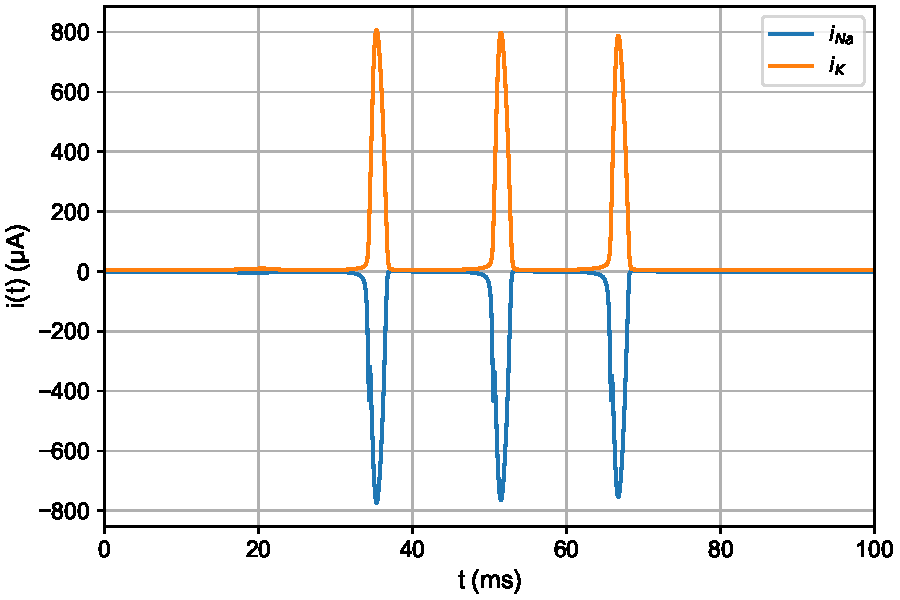
\includegraphics[width=0.9\textwidth]{figures/currents_temp6.3.pdf}
	\caption{Current densities for temperature 6.3 $^{\circ}$C}
	\label{fig:currents_temp6_3}
\end{figure}
\begin{figure}[h!]
	\centering
	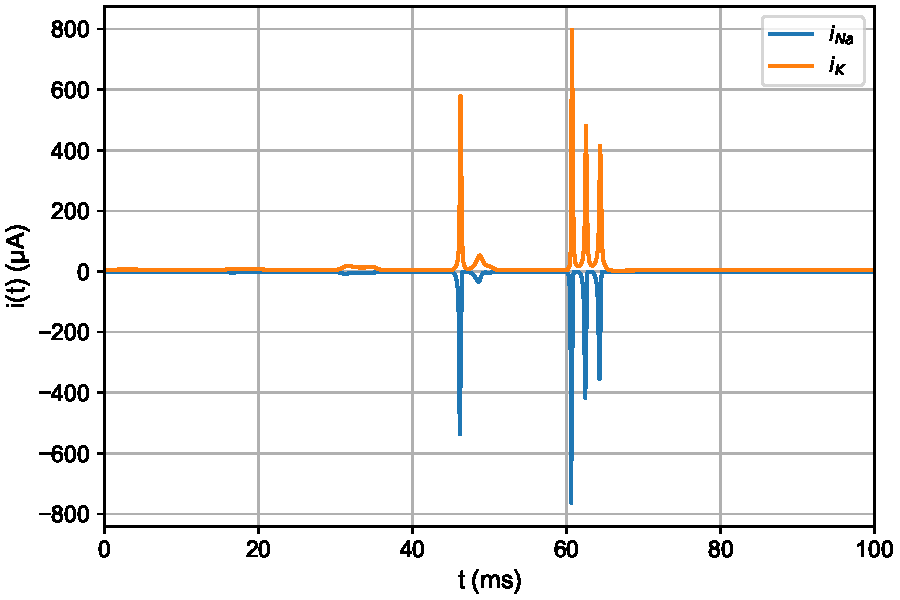
\includegraphics[width=0.9\textwidth]{figures/currents_temp28.pdf}
	\caption{Current densities for temperature 28 $^{\circ}$C}
	\label{fig:currents_temp28}
\end{figure}

\newpage
\begin{figure}[h]
	\centering
	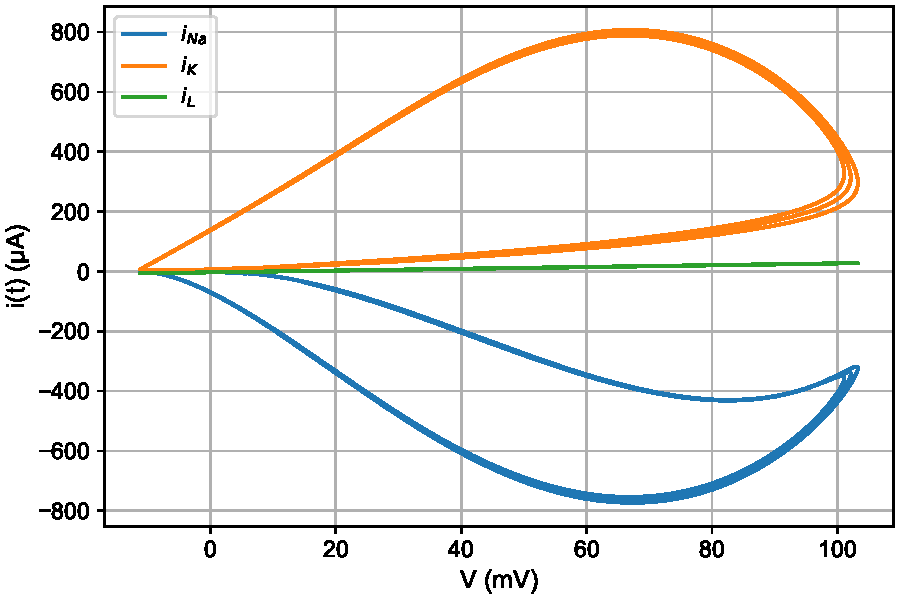
\includegraphics[width=0.9\textwidth]{figures/phase_temp6.3.pdf}
	\caption{Phase plot for temperature 6.3 $^{\circ}$C}
	\label{fig:phase_temp6_3}
\end{figure}
\begin{figure}[h!]
	\centering
	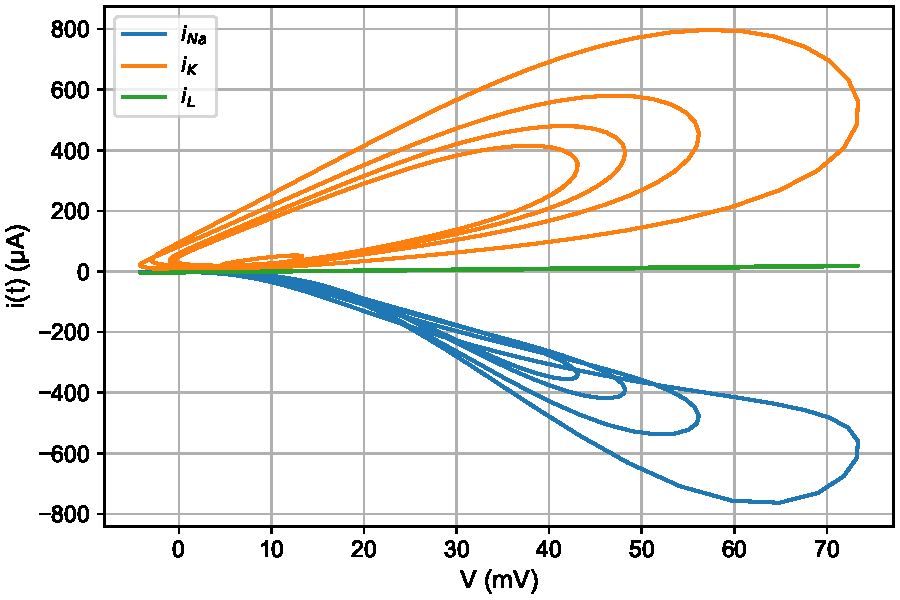
\includegraphics[width=0.9\textwidth]{figures/phase_temp28.pdf}
	\caption{Phase plot for temperature 28 $^{\circ}$C}
	\label{fig:phase_temp28}
\end{figure}

\newpage
\begin{figure}[h]
	\centering
	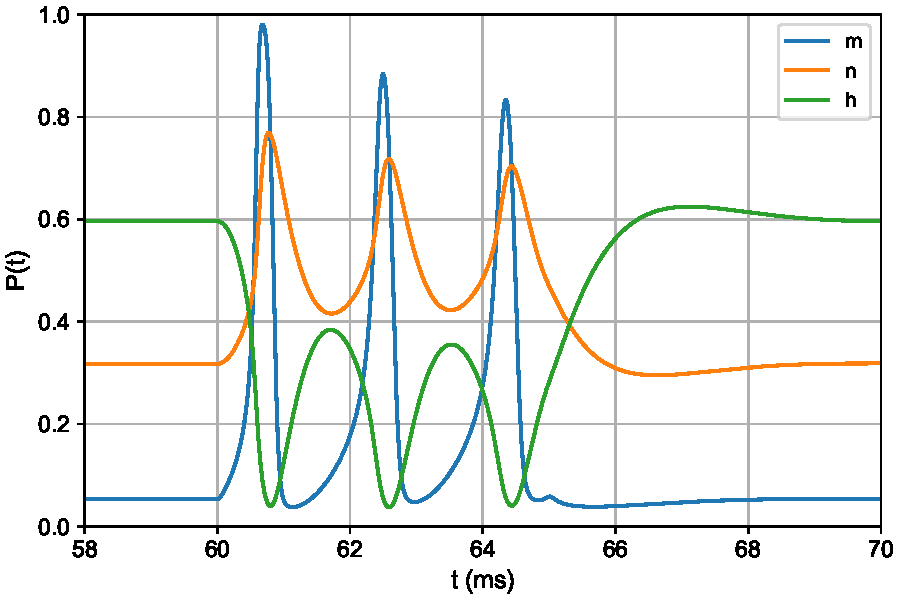
\includegraphics[width=0.9\textwidth]{figures/closeup_temp28.pdf}
	\caption{Close-up on gating variables for temperature 28 $^{\circ}$C}
	\label{fig:closeup_temp28}
\end{figure}

\end{document}